$$C(t) = C(0)\myexp{-\frac{i}{\hbar}\int_0^t\left(\frac{\hbar\omega}{2}-\frac{p^2}{2m}+\frac{1}{2}m\omega^2q^2\right)\,dt}$$
$$\dot{q}=\frac{p}{m}$$
$$\dot{p}=-m\omega^2q$$
$$\ddot{q}=\frac{\dot{p}}{m}=-\omega^2q$$
$$q(t)=A_1 e^{i\omega t} + A_2 e^{-i\omega t} $$
$$q(0)=A_1 + A_2$$
$$\dot{q}(0)=\frac{p(0)}{m}=i\omega(A_1-A_2)$$
$$A_1 = \frac{1}{2}\left(q(0)-\frac{ip(0)}{m\omega}\right)$$
$$A_2 = \frac{1}{2}\left(q(0)+\frac{ip(0)}{m\omega}\right)$$
$$q(t) = \frac{1}{2}\left(\left(q(0)-\frac{ip(0)}{m\omega}\right)e^{i\omega t}+%
			  \left(q(0)+\frac{ip(0)}{m\omega}\right)e^{-i\omega t}\right)=$$
$$=\frac{1}{2}\left(q(0)\left(e^{i\omega t}+e^{-i\omega t}\right)-%
		    \frac{ip(0)}{m\omega}\left(e^{i\omega t}-e^{-i\omega t}\right)\right)=$$
$$=q(0)\cos(\omega t)+\frac{p(0)}{m\omega}\sin(\omega t)$$
$$p(t) = m\dot{q}(t) = -m\omega q(0)\sin(\omega t) + p(0) \cos(\omega t)$$
$$\int_0^t\frac{p(t')^2}{2m}\,dt'= \frac{1}{2m}\left(p(0)^2\int_0^t\cos^2(\omega t')\,dt'+%
						     m^2\omega^2q(0)^2\int_0^t\sin^2(\omega t')\,dt'-\right.$$
$$\left.-m\omega q(0)p(0)\int_0^t2\sin(\omega t)\cos(\omega t')\,dt'\right)=$$
$$=\frac{p(0)^2}{4m}\int_0^t(1+\cos(2\omega t'))\,dt'+\frac{m\omega^2q(0)^2}{4}\int_0^t(1-\cos(2\omega t'))\,dt'-$$
$$-q(0)p(0)\int_0^t\sin(\omega t')\,d\sin( \omega t' )=$$
$$=\frac{1}{2}\left(\frac{p(0)^2}{2m}+\frac{1}{2}m\omega^2q(0)^2\right)t+%
   \frac{1}{4\omega}\left(\frac{p(0)^2}{2m}-\frac{1}{2}m\omega^2q(0)^2\right)\sin(2\omega t)-$$
$$-\frac{q(0)p(0)}{2}\sin^2(\omega t)$$
$$\frac{1}{2}m\omega^2\int_0^tq(t')^2\,dt'=\frac{1}{2}m\omega^2\left(q(0)^2\int_0^t\cos^2(\omega t')\,dt'+%
							             \frac{p(0)^2}{m^2\omega^2}\int_0^t\sin^2(\omega t')\,dt'+\right.$$
$$\left.+\frac{q(0)p(0)}{m\omega}\int_0^t2\sin(\omega t')\cos(\omega t')\,dt'\right)=$$
$$=\frac{1}{4}m\omega^2q(0)^2\int_0^t(1+\cos(2\omega t'))\,dt'+\frac{p(0)^2}{4m}\int_0^t(1-\cos(2\omega t'))\,dt'+$$
$$+q(0)p(0)\int_0^t\sin(\omega t')\,d\sin(\omega t')=$$
$$=\frac{t}{2}\left(\frac{p(0)^2}{2m}+\frac{1}{2}m\omega^2q(0)^2\right)-%
   \frac{1}{4\omega}\left(\frac{p(0)^2}{2m}-\frac{1}{2}m\omega^2q(0)^2\right)\sin(2\omega t)+$$
$$+\frac{q(0)p(0)}{2}\sin^2(\omega t)$$
$$\int_0^t\left(\frac{p(t')^2}{2m}-\frac{1}{2}m\omega^2q(t')^2\right)\,dt'=%
  \left(\frac{p(0)^2}{2m}-\frac{1}{2}m\omega^2q(0)^2\right)\frac{\sin(2\omega t)}{2\omega}-q(0)p(0)\sin^2(\omega t)$$
$$C(t) = C(0) \myexp{-\frac{i\omega t}{2}+\left(\frac{p(0)^2}{2m}-\frac{1}{2}m\omega^2q(0)^2\right)\frac{i\sin(2\omega t)}{2\hbar\omega}}$$
\begin{equation}
C(t)=C(0)\myexp{-\frac{i}{\hbar}\left(\frac{\hbar\omega t}{2}-\myl(0)\frac{\sin(2\omega t)}{2\omega}+q(0)p(0)\sin^2(\omega t)\right)}
\label{eq:coeff}
\end{equation}
%\begin{figure}[H]
%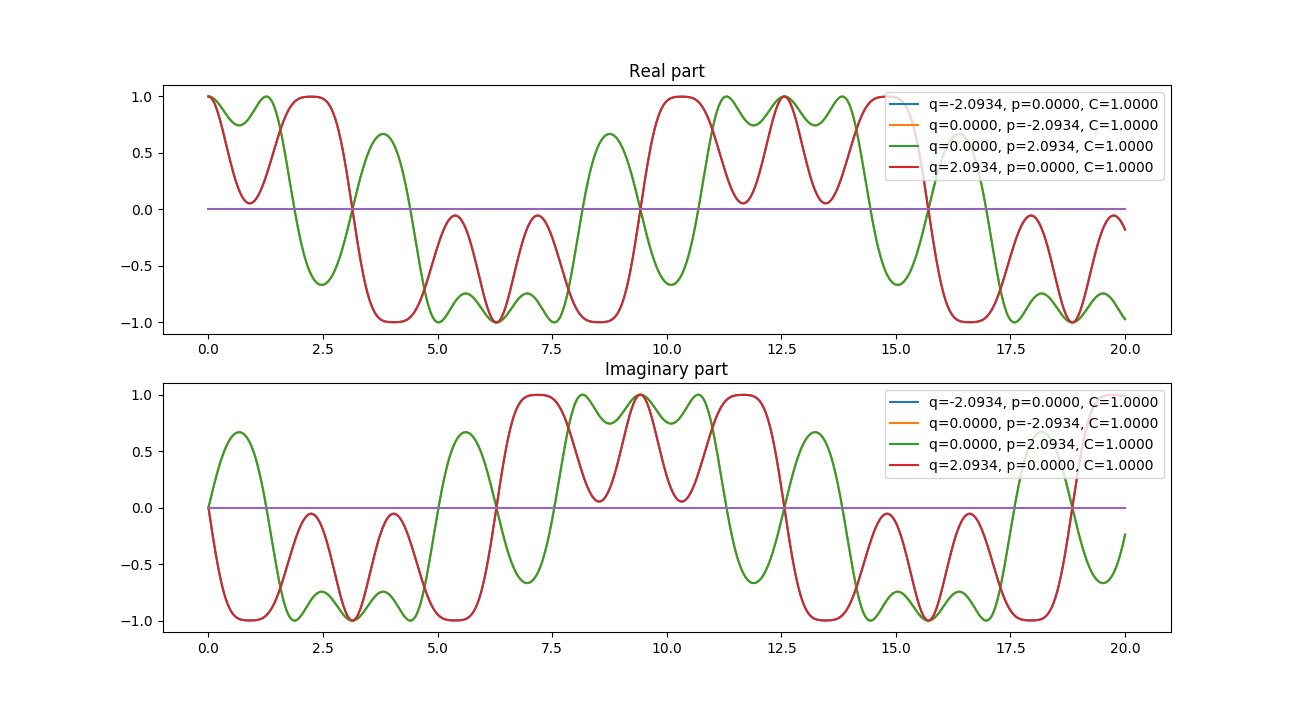
\includegraphics[scale=0.5]{eq_coeff.png}
%\caption{Вид коэффициентов (уравнение \ref{eq:coeff}), описываем состояние с энергией $2.5$ с помощью подогнанного базиса, %
%	 можем использовать базисные функции с параметром $\sim$ 0.25 и коэффициентами $[-1.0, 1.0, 1.0, -1.0]$. %
%	 Но такой сигнатуры не получаем. }
%\end{figure}
